\documentclass[12pt]{article}

\usepackage[utf8]{inputenc}
\usepackage[T1]{fontenc}
\usepackage{geometry}
\usepackage{graphicx}
\usepackage{subfig}
\usepackage{gensymb}
\usepackage{amsmath}
\geometry{a4paper}

\title{\textbf{Part 2: Basics of Gaussian Processes and Expected Improvement}}

\begin{document}
\maketitle

Hey everyone! Welcome to the first \emph{ZACLAB} post related to data science, optimization, and statistical methods. Today we will be talking about Gaussian Processes (GPs) and Expected Improvement (EI) as it relates to Bayesian Optimization (BO). I will provide code throughout the post. In fact, the majority of the material here will be in reference to code in Python that will be posted.

\section{Gaussian Processes}

Before we do anything related to BO, we have to build our own GP. A GP is a statistical way of doing regression. By statistical, I mean that by training a GP you not only get a mean but a standard deviation as well...pretty fancy! We will look at single output $\hat{\mu} \pm \hat{\sigma}$ GPs with training data $X$ and $Y$ with dimensionality $p$. There is \textbf{a lot} more to be said about GPs than this, but for now here are the two most important equations for GPs to understand:

\begin{equation}
\hat{\mu} = K(x,X)(K(X,X) + \sigma^{2}I)^{-1}Y
\end{equation}
\begin{equation}
\hat{\sigma}^{2} = K(x,x) - K(x,X)(K(X,X)^{-1}K(X,x)
\end{equation}

Next we must understand that $K$ object. It's a matrix called a kernel. It is a mathematical relationship, in this case between two stationary points, say $x_{i}$ and $x_{j}$ with something like the squared exponential kernel... $K(x_{i},x_{j}) = \sigma_{f}^{2}exp(-r/2*l^{2})$ where $r = ||x_{i}-x_{j}||_{2}^2$ (or the squared L2 norm of the difference between $x_{i}$ and $x_{j}$. 

\vspace{5mm}

So let's apply the GP to a toy problem... $f(x) = x_{1}-x_{2}+U(0,0.1)$ as shown in Figure 1. The black crosses is the data $X$ associated with a given $Y$ we will be working with. To apply the GP, calculate $\hat{\mu}$ for any point $x_1,x_2$ you want using the training data $X,Y$; that is, calculate $K(X,X)$ for your data and calculate $K(x,X)$ for any $x$ you want to predict $\hat{\mu}$ and $\hat{\sigma}$.

\begin{figure}
\centering
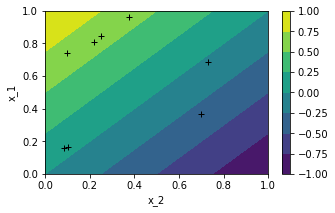
\includegraphics[width=0.7\textwidth]{Post_2_fcontour}
\caption{Toy Function}
\end{figure}

\section{Hyperparameter Optimization for GPs}

Something I forgot (intentionally) to mention in Section 1 was that GPs, while not having structure such as in linear or quadratic models, have hyperparameters. These are parameters that control how the GP behaves. In our example, the squared exponential kernel has three hyperparameters: a model error parameter $\sigma$, an amplitude parameter $\sigma_{f}$, and a length scale parameter $l$. We can define a likelihood function $L(\sigma,\sigma_{f},l)$ based on these parameters.

\begin{equation}
L(\sigma,\sigma_{f},l) = -0.5YK_{y}Y^{T} - 0.5log(det(K_{y}))-0.5nlog(2\pi)
\end{equation}

\begin{equation}
K_{y} = (K(X,X,\sigma_{f},l)+\sigma^{2}I)^{-1}
\end{equation}

We can plot slices of $L$ for the parameters in our problem as shown in Figure 2. We will talk about three different ways to get the optimal hyperparameters for this GP, (1) random search, (2) gradient descent method, and (3) BFGS method.

\begin{figure}
\centering
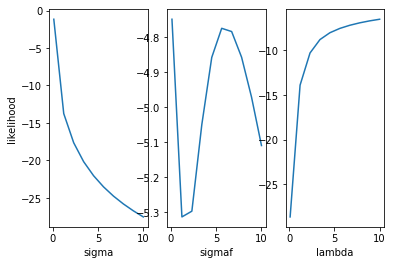
\includegraphics[width=0.7\textwidth]{Post_2_hyperresults}
\caption{Likelihoods for Various Hyperparameters}
\end{figure}

\subsection{Random Search}

The simplest way of getting optimal hyperparameters is to randomly search for them. This one is simple because it does not rely on gradients. I just calculate $L$ for $M = 100$ random hyperparameters $[0.1,20]$ and use the smallest $L$ result.

\subsection{Gradient Descent Method}

Next we will use gradient information to improve search. We'd do this if the number of hyperparameters is large. The gradient of the likelihood function $L$ is as follows:

\begin{equation}
\nabla L = (\nabla L_{\sigma}, \nabla L_{\sigma_{f}}, \nabla L_{l}) = 0.5 Tr(\alpha \alpha^{T} - K_y^{-1} \nabla_{i}L)
\end{equation}

\begin{equation}
\nabla_{\sigma} L = 2\sigma I
\end{equation}

\begin{equation}
\nabla_{\sigma_{f}} L = 2/\sigma_{f} K(X,X)
\end{equation}

\begin{equation}
\nabla_{l} L_{i,j} = K(x_{i},x_{j}) r(x_{i},x_{j}) / l^{3}
\end{equation}

\begin{equation}
\alpha = K_y^{-1} Y
\end{equation}

The update scheme for gradient descent will be $\theta_{k+1} = \theta_{k} + \eta \nabla L$ where $\eta = 0.1$ for hyperparameters $\theta$. Using a random initialization of the hyperparameters and $M = 1000$ iterations of gradient descent, we get the results shown in Figure 2(b). For those of you familiar with gradient descent, we use $-\nabla L$ rather than $\nabla L$ for our optimal step because we are maximizing $L$ rather than minimizing. Note also that our hyperparameters $\theta$ must be $>0$ so we modify our gradient descent to be \emph{projected} gradient descent. Simply, if a constraint is violated we project the violated parameter onto the viable set $\Theta$; in this case $\theta = 0$. An example is shown in Figure 3.

\begin{figure}
\centering
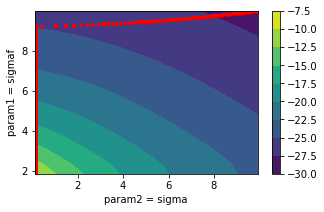
\includegraphics[]{Post_2_gpresults}
\caption{Gradient Descent \emph{in Action!}}
\end{figure}

\subsection{BFGS Method}

The final thing I'd like to talk about with hyperparameter optimization is using the BFGS gradient method to solve the optimization problem. BFGS stands for \emph{Broyden–Fletcher–Goldfarb–Shanno} and approximates the Hessian $\nabla^2 L$ of the objective function to speed up optimization. Here we will implement BFGS using \emph{sci-py}'s \emph{scipy.optimize.minimize} program. Just make sure to pass $X$ and $Y$ as constants to the optimizer so $L$ and $\nabla L$ can be calculated, which can be done (and is done in the code) using wrapper functions. Additionally, just like projecting the failed gradients onto the feasible space $\Theta$, we must tell \emph{scipy.optimize.minimize} we have upper and lower bounds.

\begin{figure}
\centering
\subfloat[][Random]{
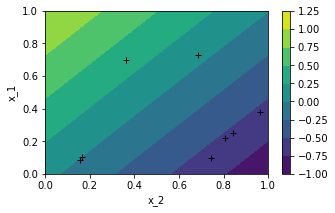
\includegraphics[width=0.3\textwidth]{Post_2_fcontour_rand}}
\subfloat[][Gradient Descent]{
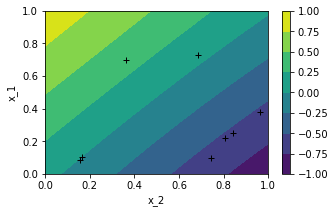
\includegraphics[width=0.3\textwidth]{Post_2_fcontour_gd}}
\subfloat[][BFGS]{
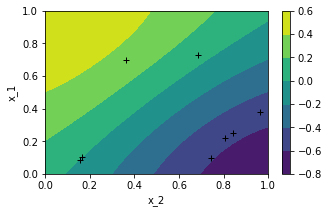
\includegraphics[width=0.3\textwidth]{Post_2_fcontour_bfgs}}
\caption{Results for Hyperparameter Optimization Methods}
\end{figure}

\section{Expected Improvement}

Next we implement a useful tool for optimization. It a function called \emph{Expected Improvement} (EI), which is a way to optimize a random objective function mean $\hat{\mu}$ with uncertainty $\hat{\sigma}^2$. We will use it to design intelligent experiments, which will be a common theme in many of these posts. For example, if we have chemicals in concentrations $X$ and cost $Y$ for each combination, we will solve the problem:

\begin{equation}
X^* = argmin\:\mu(X)
\end{equation}

\vspace{5mm}

Where experimental data has been collected and modeled using a GP. As before, without going into too much detail, here is the basic equation for single-output EI where a single set of inputs is suggested ($q=1$). Note that $\Phi$ and $\phi$ is the CDF and PDF of the standard normal distribution respectively. 

\begin{equation}
EI(X) = (Y_{min}-\hat{\mu})\Phi(z) - \hat{\sigma}\phi(z)
\end{equation}

\begin{equation}
z =  (Y_{min}-\hat{\mu})/\hat{\sigma}
\end{equation}

In the figures below we show a contour plot of some experiments with GP model standard deviations and it's respective EI plot. Note that in the minimization setting, the best region is on the lower right, but there is uncertainty in both lower right and upper left. The EI distinguishes the two and biases towards the lower right \textbf{as wanted}. This is valuable in expensive optimization processes where the question of which parameters to evaluate next is non-trivial and/or expensive.

\begin{figure}
\centering
\subfloat[][Standard Deviation]{
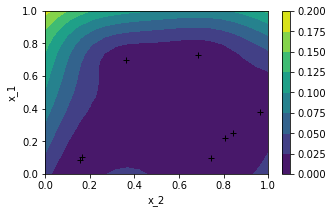
\includegraphics[width=0.4\textwidth]{Post_2_uncertainty}}
\subfloat[][Expected Improvement]{
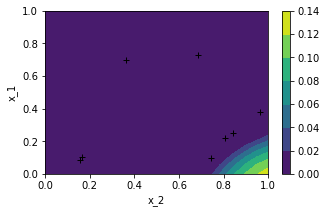
\includegraphics[width=0.4\textwidth]{Post_2_EI}}
\end{figure}

\section{EI and \emph{Botorch}}

We end this post with a discussion (and code posted) about \emph{Botorch}. This is a robust Python implementation of a lot of what we have talked about. I have just written simple code to create a GP similar to what we did above, and optimize it's parameters using BFGS. In Figure 5(a) the contour looks similar to ours, and in Figure 5(b) the regressive predictions for $M=1000$ random predictions on the toy problem largely adhere to the $45\degree$ line in black.

\begin{figure}
\centering
\subfloat[][\emph{Botorch} GP]{
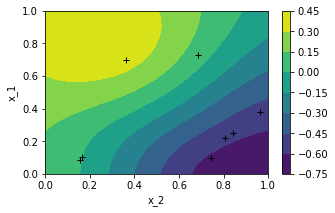
\includegraphics[width=0.4\textwidth]{Post_2_fcontour_bo}}
\subfloat[][Regressive Plots]{
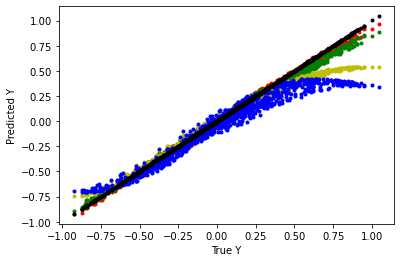
\includegraphics[width=0.4\textwidth]{Post_2_truevspredict}}
\caption{Model Comparison and \emph{Botorch}}
\end{figure}

\vspace{5mm}

We this was fun! Next week we'll be talking about radial basis functions!

\end{document}